% Template for a Computer Science Tripos Part II project dissertation
\documentclass[12pt,a4paper,twoside,openright]{report}
\usepackage[pdfborder={0 0 0}]{hyperref}    % turns references into hyperlinks
\usepackage[margin=25mm]{geometry}  % adjusts page layout
\usepackage{amsmath} % For masthy things
\usepackage{graphicx}  % allows inclusion of PDF, PNG and JPG images
\usepackage{docmute}   % only needed to allow inclusion of proposal.tex
\usepackage{fancyvrb} % Verbatim environment with samepage=true argument produces useful code listings restricted to the same page
\usepackage{color} % Uses color to remind me of things to do.
\usepackage{wrapfig} % used for wrapping text around images

\graphicspath{ {figs/} }

\raggedbottom                           % try to avoid widows and orphans
\sloppy
\clubpenalty1000%
\widowpenalty1000%

\renewcommand{\baselinestretch}{1.1}    % adjust line spacing to make
                                        % more readable

\begin{document}

\bibliographystyle{plain}


%%%%%%%%%%%%%%%%%%%%%%%%%%%%%%%%%%%%%%%%%%%%%%%%%%%%%%%%%%%%%%%%%%%%%%%%
% Title


\pagestyle{empty}

\rightline{\LARGE \textbf{Robin McFarland}}

\vspace*{60mm}
\begin{center}
\Huge
\textbf{Giving Programming Exercises Adaptive Difficulty} \\[5mm]
Computer Science Tripos -- Part II \\[5mm]
Homerton College \\[5mm]
2017
\end{center}

%%%%%%%%%%%%%%%%%%%%%%%%%%%%%%%%%%%%%%%%%%%%%%%%%%%%%%%%%%%%%%%%%%%%%%%%%%%%%%
% Proforma, table of contents and list of figures

\pagestyle{plain}

\chapter*{Proforma}

{\large
\begin{tabular}{ll}
Name:               & \bf Robin McFarland                       \\
College:            & \bf Homerton College                     \\
Project Title:      & \bf Giving Programming Exercises Adaptive Difficulty \\
Examination:        & \bf Computer Science Tripos -- Part II, July 2017  \\
Word Count:         & \bf TBC  \\
Project Originator: & Mr Michael B.~Gale                   \\
Supervisor:         & Mr Michael B.~Gale                    \\ 
\end{tabular}
}

\section*{Original Aims of the Project}


\section*{Work Completed}

\section*{Special Difficulties}
 
\newpage
\section*{Declaration}

I, Robin McFarland of Homerton College, being a candidate for Part II of the Computer
Science Tripos, hereby declare
that this dissertation and the work described in it are my own work,
unaided except as may be specified below, and that the dissertation
does not contain material that has already been used to any substantial
extent for a comparable purpose.

\bigskip
\leftline{Signed [signature]}

\medskip
\leftline{Date [date]}

\tableofcontents

\listoffigures

\newpage
\section*{Acknowledgements}

\pagestyle{headings}

\chapter{Introduction}

\textcolor{red}{MiniJava is a language I have developed.}

\chapter{Preparation}

\textcolor{red}{
\begin{itemize}
\item{First attempt using Strings}
\item{Why I had to make my own language}
\item{Research into other projects etc, like Arjen and the PhD}
\end{itemize}
}

Since part of my aim was to demonstrate a possible method for teaching Java, I wanted the language I was using to be as close to Java as possible. However, re-implementing all of Java would have been too much unnecessary complexity, so I designed MiniJava with reference to only a small subset of the Java 8 grammar \cite[p.714]{Java8}. Since nodes in the AST represent constructs in the source code, replacing a node in the AST with a notional ``blank'' node would be representative of making parts of the source code blank. 

\textcolor{red}{"Are there any limitations of using antlr and how it compared to other parser generators / techniques"}

%%%%%%%%%%%%%%%%%%%%%%%%%%%%%%%%%%%%%%%%%%%%%%%%%%%%%%%
% Implementation chapter
\chapter{Implementation}

\textcolor{red}{("it feels a lot like you are explaining the code with the expectation that the reader is looking at the code and reads your description alongside it, when you should really be explaining how it works and what the intuition is (note: explaining how something works is not the same as explaining the code)")}

\textcolor{red}{("You should be approaching the write-up from the perspective of "how do I explain the problems and solutions to someone who has never seen anything about this project before", don't go through the code, pick parts, and describe those.")}

In this chapter I detail the work completed. I begin by describing how I implemented MiniJava, (a small imperative programming language based on Java), as well as a parser for MiniJava's grammar. I then describe the algorithm that allows the addition and removal of ``blanks'' within a MiniJava program. I then describe how a programming exercise is conceptualised in the abstract sense, and give an example of an implementation of a specific question. Finally, I describe the two peripherals I developed to interact with the language; the \texttt{ExerciseSetter} and the Graphical User Interface (GUI).

\section{MiniJava's Abstract Syntax Tree}

In this section I describe the implementation of the MiniJava language.

Each class in my implementation represents a different production rule in the abstract syntax for MiniJava, found in Appendix \ref{App:Parser} in the form of a parser specification. In order to allow other parts of my code to operate on instances of these classes without needing to know exactly what they are, every class in the implementation implements the \texttt{MiniJASTNode} interface. This acts as the top of the object hierarchy for my implementation. 

It is important to differentiate between MiniJava expressions and MiniJava statement as they must be used in different places. For example, in the production rule \texttt{WHILE~parExpression~statement} representing a \texttt{while} loop, \texttt{parExpression} may be substituted with any MiniJava expression (surrounded by parentheses), while \texttt{statement} may be substituted with any MiniJava statement. The reverse is not allowed however, meaning that \texttt{statement} may not be replaced by a MiniJava expression and vice versa. This distinction is made by the interfaces \texttt{Expression} and \texttt{Statement} (which all MiniJava expressions and statements implement respectively), and the abstract classes \texttt{ExpressionBase} and \texttt{StatementBase} (which all MiniJava expressions and statements extend respectively). Both interfaces and abstract class are used here because of the need to include blanks in the grammar. There are two classes representing blanks: \texttt{FillableBlankExpr} and \texttt{FillableBlankStmnt}. The first of these should be a MiniJava expression and the second should be a MiniJava statement, meaning they should extend \texttt{ExpressionBase} and \texttt{StatementBase} respectively, but both of them must also extend the abstract class \texttt{FillableBlank} (this is explained on page \pageref{Para:Blanks}). Since classes in Java cannot extend more than one base class, the only alternative is for them to implement the \texttt{Expression} and \texttt{Statement} interfaces. However, removing \texttt{ExpressionBase} and \texttt{StatementBase} would result in too much repeated code across the whole grammar, so the grammar requires both the interfaces and the abstract classes. The enumeration \texttt{SingleWordStmnt} (each value of which represents a MiniJava statement that is trivial, consisting of zero or one word) must also be a MiniJava statement, and since enumerations cannot extend classes, it must implement \texttt{Statement}, further cementing the need for both the interfaces and the abstract classes. Since the distinction between expressions and statements is the most high level distinction one can make, both the \texttt{Expression} and \texttt{Statement} interfaces extend the \texttt{MiniJASTNode} interface, ensuring that every class in the implementation also implements it.

As important as the distinction between expressions and statements is, there do exist some expressions that can be used in statements. For an example, the MiniJava code \texttt{i~=~5;} is a statement because it ends in a semicolon,~``\texttt{;}'', but this statement consists entirely of the expression \texttt{i~=~5} (this allows for the chaining of assignments found in the Java grammar \cite[p.589]{Java8}). This sort of expression within a statement construct is not possible with all expressions, for example the code \texttt{i~+~4;} would not be valid MiniJava. To make the distinction between expressions which may be used in statements like this and those which may not, I made the interface \texttt{StatementExpression}. This interface is only implemented by those expressions which can be used in a statement this way.

A feature of MiniJava is the concept of operator precedence, which is used to disambiguate an otherwise ambiguous grammar of expressions. Without the concept of operator precedence, the code \texttt{1~+~2~*~3} is ambiguous, as it can be read as either \texttt{(1~+~2)~*~3} which equates to 9, or as \texttt{1~+~(2~*~3)} which equates to 7. Since a single arithmetic expression cannot have more than one value, a decision must be made as to which of these interpretations is declared valid. The decision taken aligns with the standard arithmetic order of operations, such that the answer of 7 is the correct answer in this case. This example demonstrates that the multiplication operator, ``\texttt{*}'', has a higher precedence than the addition operator, ``\texttt{+}''. All the possible operators in MiniJava are found within this precedence hierarchy, and I needed some way to encode this. The method I chose for this is the natural choice, since it is suggested by the Java grammar itself \cite[p.723]{Java8}. The production rule for \texttt{AdditiveExpression} is as follows:
\begin{Verbatim}[samepage=true]
AdditiveExpression:
    MultiplicativeExpression                        (1)
    AdditiveExpression + MultiplicativeExpression   (2)
    AdditiveExpression - MultiplicativeExpression   (3)
\end{Verbatim}
and the production rule for \texttt{MultiplicativeExpression} is as follows:
\begin{Verbatim}[samepage=true]
MultiplicativeExpression:
    UnaryExpression
    MultiplicativeExpression * UnaryExpression
    MultiplicativeExpression / UnaryExpression 
    // Note that the modulus operator, %, was removed from MiniJava
\end{Verbatim}
This means that for any expression $A$\texttt{ + }$B$, the expression $A$ must only contain subexpressions that use operators with precedence at least as high as \texttt{+} and \texttt{-}, and $B$ must only contain subexpressions that use operators with precedence higher than \texttt{+} and \texttt{-}. For any expression $A$\texttt{ * }$B$, neither $A$ nor $B$ can contain subexpressions that use operators with precedence lower than \texttt{*} and \texttt{/}. This in turn indicates that an expression such as \texttt{1~+~2~*~3~+~4} can only be interpreted as \texttt{1~+~(2~*~3)~+~4}, and an expression such as \texttt{1~*~2~+~3~*~4} can only be interpreted as \texttt{(1~*~2)~+~(3~*~4)}. I wanted an operator precedence for MiniJava that is hardcoded within the grammar of MiniJava itself, just as the operator precedence of Java is hardcoded within the grammar of Java. The production rules for Java shown above suggest a natural implementation of the class that represents addition expressions:
\begin{Verbatim}[samepage=true]
class AddExpr {
    private boolean isPlus;
    private AddExpr leftSide;
    private MultExpr rightSide;
    ...
}
\end{Verbatim}
Here, the \texttt{isPlus} field records whether the expression is an addition or a subtraction, \texttt{leftSide} and \texttt{rightSide} store the left and right operands of the expression, and \texttt{MultExpr} is the class representing multiplication expressions. What has been implemented so far encapsulates parts (2) and (3) of the \texttt{AdditiveExpression} production rule above, but not part (1). This part is encapsulated by making the class \texttt{MultExpr} extend the class \texttt{AddExpr}, such that an instance of \texttt{MultExpr} may always be used in place of an instance of \texttt{AddExpr}. Note that since multiplication operators are higher in the operator precedence hierarchy, their representations are lower in the object hierarchy. This then is the solution to the operator precedence problem: to enforce an operator precedence hierarchy, first enforce an inverse object hierarchy in their representative classes, and then choose the type of each expression's operands to match the relevant terminal symbols in the relevant production rule.\footnote{Note that if you were to look at my implementation of \texttt{AddExpr}, \texttt{leftSide} and \texttt{rightSide} would both be \texttt{int}s, not \texttt{AddExpr} and \texttt{MultExpr} instances. The reason behind this is explained in section \ref{Sec:Blanks}.}

\begin{figure}
\centering
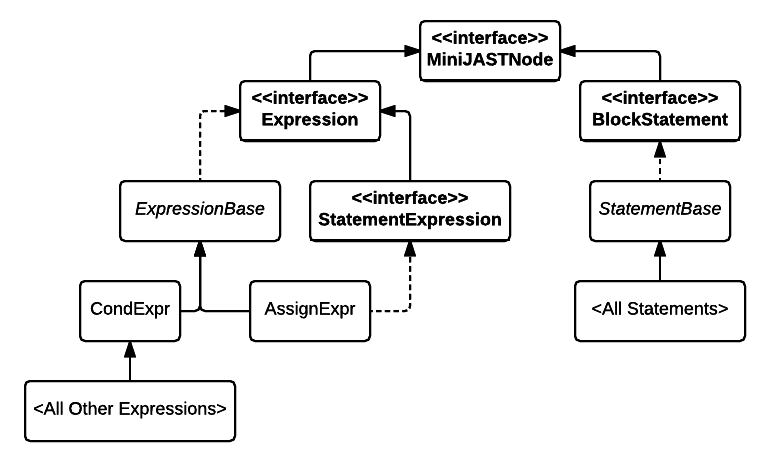
\includegraphics{TopLevelUML}
\caption{The UML diagram showing the top of the object hierarchy for \texttt{MiniJASTNode}s.}
\label{Fig:UML}
\end{figure}

Figure \ref{Fig:UML} shows the top of the object hierarchy for the implementation of MiniJava. It demonstrates the distinction between MiniJava expressions and statements by way of the \texttt{Expression} and \texttt{Statement} interfaces, the extra classification of expressions that can be used as statements given by \texttt{StatementExpression}, and shows the beginnings of the operator precedence hierarchy hardcoded into the expressions.

Note also that as a side-effect of this implementation, the ambiguous code \texttt{1~+~2~+~3} also only has one possible interpretation, namely \texttt{(1~+~2)~+~3}. This follows the established rules of operator associativity, which are now also hardcoded into the grammar.

In MiniJava, every expression has a type which consists of a primitive type and may or may not be an array type. There are four possible primitive types: \texttt{boolean}, \texttt{char}, \texttt{int}, and \texttt{double}. The primitive types are represented in the grammar by the enumeration, \texttt{PrimType}. The type of an expression then is represented by the class \texttt{Type}, an instance of which stores the appropriate PrimType value and a flag determining whether or not it is an array type. These \texttt{Type}s are use by the interpreter to determine whether or not variables can contain certain values, and whether operators are being supplied with the appropriate operands.

The majority of statements in MiniJava are composed of statements or expressions, but there are some that consist of only a single word, or even no words at all. To have an entire class representing each of these trivial statements seems wasteful, so the enumeration \label{Para:SingleWordStmnt}\texttt{SingleWordStmnt} represents four such statements: the break statement (\texttt{break;}), the continue statement (\texttt{continue;}), the return statement (\texttt{return;}), and the empty statement (\texttt{;}). Although there are no functions in the MiniJava grammar, the return statement can be used to immediately halt evaluation.

As we have seen previously, \texttt{AddExpr} defines the boolean field \texttt{isPlus}, to determine whether this instance represents an addition or a subtraction. There are some expressions where the number of possible operators that can be used in that expression is greater than two, in which case a boolean field will not be enough to disambiguate. \texttt{RelationExpr} and \texttt{AssignExpr} are the two expressions for which this is the case, since there are four relation operators and five assignment operators. These possible operators are represented by the two enumerations \texttt{RelationOp} and \texttt{AssignOp}. Thus \texttt{RelationExpr} stores a value of \texttt{RelationOp}, and \texttt{AssignExpr} stores a value of \texttt{AssignOp}.

There are two possible MiniJava expressions that can be assigned to, i.e. they can appear on the left hand side of an assignment expression. These two, identifiers and array accesses, are represented by the classes \texttt{Id} and \texttt{ArrayAccess}. To signify that they can both be assigned to, both classes implement the \texttt{AssignLHS} interface, an interface used for only this purpose. Similarly, there are two possible MiniJava expressions that can be assigned to an array type variable. These are array creation expressions (for example \texttt{new int[4]}) and array initialisation expressions (for example \texttt{\{1, 2, 3, 4\}}), which are represented by the classes \texttt{arrayCreation} and \texttt{ArrayInit} respectively. To signify that both can be assigned to arrays, they both extend the abstract class, \texttt{ArrayAssignRightSide}. To justify why \texttt{AssignLHS} is an interface and \texttt{ArrayAssignRightSide} is an abstract class, we consider the difference between the expressions that can appear as subexpressions of other expressions, and those that cannot. Identifiers and array accesses may appear as a subexpression of some other expression. Because of this, the index operator used in array accesses must appear within the operator precedence hierarchy described previously, and so too must identifiers. If identifiers were not present in the operator precedence hierarchy, then they could never be substituted for the terminal symbols in the production rules seen previously, ruling out valid expressions like \texttt{i~+~j}. If identifiers and array accesses must appear in the operator precedence hierarchy, and high up in it too, then that means their representative classes must extend some class representing an operator lower down in the hierarchy. Thus \texttt{AssignLHS} must be an interface and not an abstract class, as \texttt{Id} and \texttt{ArrayAccess} already subclass some other class (namely \texttt{UnaryExpr}). Array creation and initialisation expressions however can never appear as a subexpression of some expression (since only single-dimensional arrays are allowed, expressions such as \texttt{\{\{1\},\{2,3,4\}\}} are not valid). This means that they do not appear in the operator precedence hierarchy, and thus their representations do not need to extend any base class. Thus \texttt{ArrayAssignRightSide} can usefully be an abstract class, reducing the amount of repeated code in these two classes.

MiniJava uses local variable declarations (for example, \texttt{int i = 4, ar[];}) in the same way that Java does: to declare and initialise new variables. Local variable declarations can be thought of as being made up of a primitive type and a list of so called ``variable declarators'', which are identifiers that may or may not be followed by square brackets to show the new variable is an array, and which may or may not be followed by an equals sign, ``\texttt{=}'', and a value with which to initialise the new variable. My implementation represents local variable declarations using the class \texttt{LocalVarDec}, which consists of a \texttt{PrimType} and a list of \texttt{VarDeclarator} instances. The \texttt{VarDeclarator} class stores a String containing the name of the variable, flags to determine whether the variable is an array type and whether an initialiser expression is given, and the initialiser expression itself if there is one.

What distinguishes MiniJava from other languages is that the concept of a blank, a missing piece of code, is built into the grammar itself. \label{Para:Blanks} Representations of blanks in code should enable a user to fill one with their own code. To do this programmatically, it is necessary for representations of blanks to each come with a unique id, such that users can choose which blank they are filling and the blank be searchable within the AST representing the program. The abstract class \texttt{FillableBlank} fulfils this requirement by storing a \texttt{static} reference to an \texttt{AtomicInteger} and a private \texttt{int} field, \texttt{id}. Whenever a new blank needs to be represented in an AST, an instance of a class that extends \texttt{FillableBlank} can be supplied with a unique identifier that has not yet been used in this runtime environment, by using the \texttt{AtomicInteger}'s \texttt{incrementAndGet} method and storing the result in \texttt{id}. The two concrete classes that extend \texttt{FillableBlank} are \texttt{FillableBlankExpr} and \texttt{FillableBlankStmnt}. The first of these can be used to replace a MiniJava expression (and thus implements the \texttt{Expression} interface so that it can be stored in a MiniJava AST), and the second can replace a MiniJava statement (and thus implements \texttt{Statement}). \texttt{FillableBlankExpr} stores an \texttt{Expression} field, \texttt{studentExpr}, which, if not \texttt{null} is representative of the code with which a user has filled the blank. Similarly, \texttt{FillableBlankStmnt} stores an \texttt{Statement} field, \texttt{studentStmnt}.

In this section I have described the implementation of my MiniJava language.

\section{Interpreting the language}

In this section I explain how MiniJava programs are interpreted.

To correctly interpret MiniJava, several requirements must be met by the interpreter:
\begin{enumerate}
\item{The scope of variables must be handled, such that when a variable is used its current value can be accessed, and the same variable can't be declared twice in one scope.}
\item{Expressions must be able to propagate their values upwards, so that surrounding expressions and statements can use them.}
\item{Flow control must be handled, such that break and continue statements can be used in loops.}
\item{If an exception is raised during execution, the exception should propagate up and halt execution, preferably delivering a useful message.}
\end{enumerate}

The scope of variables is handled by the interpreter with instances of the \texttt{Context} class. Part of its definition is shown below:
\begin{Verbatim}[samepage=true]
public class Context {
    public Stack<HashMap<String, Type>> namesToTypes;
    public Stack<HashMap<String, Object>> namesToValues;
    ...
}
\end{Verbatim}
The \texttt{namesToTypes} field is a stack of maps from names (as \texttt{String} values) to instances of my \texttt{Type} class. Every variable that is declared in this scope will have an entry in the map on top of this stack, recording the type of that variable. The \texttt{namesToValues} field is a stack of maps from names to instances of \texttt{Object}. If a variable has an entry in the map on top of this stack, then the variable has the value stored in the map with it in this scope. It is possible for a variable to have an entry in the map on top of the \texttt{namesToTypes} stack, but not in the map on top of the \texttt{namesToValues} stack: this indicates that the variable has been declared but not initialised in this scope.

During execution, the interpreter must keep track when variables will go out of scope. This is handled by the \texttt{stepIn} and \texttt{stepOut} methods in \texttt{StatementBase}. The \texttt{stepIn} method is called whenever execution enters a new, deeper, scope. This method copies every key value pair in the maps on top of their respective stacks into new maps, and pushes these new maps onto the stack. Thus every entry in one of the stacks represents a different scope: as you move down the stack, you move outward through the nested scope. The \texttt{stepOut} method is called whenever execution leaves the current scope. At this point, all the variables that do not exist in the new scope should be forgotten, and every variable that does exist in this new scope should have their value updated to the value it was in the old scope. The \texttt{stepOut} method first pops the top off both stacks, storing the top of the \texttt{namesToValues} stack in the local variable \texttt{oldMap}. Then, for every key in \texttt{oldMap}, if this key also appears in the new top of the \texttt{namesToTypes} stack, the corresponding value in \texttt{oldMap} is used to update the top of the \texttt{namesToValues} stack. In this way, variables can be updated in deeper levels of scope, and retain their new values when execution moves up the nested scope.

Consider the expression \texttt{(2*3)+4}. In MiniJava, this expression might be represented by a \texttt{AddExpr} storing a literal with the value \texttt{4} as the right operand, and an \texttt{MultExpr} as the left operand. This \texttt{MultExr} would store literals with values \texttt{2} and \texttt{3} as the left and right operands. During the evaluation of an expression, the most deeply nested parts of the expression must be evaluated first, so that their values can be used further up in the nested expression. There is no point trying to evaluate the \texttt{AddExpr} before we know the value of \texttt{(2*3)}. Thus, the \texttt{MultExpr} needs a way to communicate to the \texttt{AddExpr} that it has a value of \texttt{6}, so that the \texttt{AddExpr} can be evaluated to \texttt{10}. Likewise, whatever context the \texttt{AddExpr} is in needs to be told it has the value \texttt{10}. The way this is done in MiniJava is using implementations of the \texttt{ReturnValues} abstract class. This class represents the notion that some value is being returned by an expression, but allows any type of value to be returned, no matter what primitive type the value takes, and whether it's an array or not. To return a value of a particular primitive type, the appropriate one of these four implementations must be used: \texttt{ReturnValuesBool}, \texttt{ReturnValuesChar}, \texttt{ReturnValuesInt}, or \texttt{ReturnValuesDouble}. Each of these has a public \texttt{value} field of the appropriate type. If an array value is being returned by an expression, then a further implementation of \texttt{ReturnValues} must be used, the generic class \texttt{ReturnValuesArray<T>}. This class makes use of Java Generics as it stores an internal \texttt{ArrayList<T>} of values.

In the same way that MiniJava expressions dispense values, MiniJava statements dispense control flow commands. These commands can be to ``break'', to ``continue'', to ``return'', or there can be no command, in which case execution continues as normal. The MiniJava interpreter represents these commands using the \texttt{FlowControl} enumeration, which has the four values \texttt{BREAK}, \texttt{CONTINUE}, \texttt{RETURN}, and \texttt{NONE}. Whenever a statement is executed, the interpreter looks for which value is dispensed and reacts accordingly. 

Several custom exceptions are used by the interpreter, to differentiate between when an error occurs in the MiniJava program being interpreted, and when an error occurs in the interpreter itself. All these custom exceptions subclass the base class of \texttt{MiniJavaException}, and the majority of them are analogous to standard Java exceptions. For example, the \texttt{OutOfBoundsException} is thrown by the interpreter whenever an index is used in an array where no such index exists. This exception is analogous to Java's \texttt{IndexOutOfBoundsException}.

The MiniJava interpreter is implemented using the \texttt{evaluate} method in the \texttt{Expression} interface, and the \texttt{execute} method in the \texttt{Statement} interface. The method signatures of these two methods are shown below:
\begin{Verbatim}[samepage=true]
public interface Expression extends MiniJASTNode {
    ReturnValues evaluate(Context c) throws MiniJASTException;
    ...
}

public interface Statement extends MiniJASTNode {
    FlowControl execute(Context c) throws MiniJASTException;
    ...
}
\end{Verbatim}
It can be seen that the interpreter makes use of all the components meeting the requirements for the interpreter. The \texttt{evaluate} method is overridden by every class representing a MiniJava expression, and the \texttt{execute} method is overridden by every class representing a MiniJava statement. This means that both methods are recursive: expressions being evaluated will call the \texttt{evaluate} method on their subexpressions for example. Typically, execution is initiated with an empty \texttt{Context} object that becomes more populated as more variables are declared. This interpreter can also be plugged in to peripherals. The values of variables in the outermost scope can be accessed after execution has terminated, and MiniJava has an inbuilt print statement, represented by the class \texttt{PrintStatement}, that can print the values of expressions to a file. Peripherals could also, if they wanted, make use of the custom exceptions thrown during execution, and the initial \texttt{Context} object.

It is important to remember that the MiniJava grammar also contains the notion of blanks in code, and thus the interpreter must be equipped to deal with these appropriately. If a blank has not yet been filled, then the interpreter should throw a custom exception, but if the blank has been filled, then execution must continue as if there was no blank there. The \texttt{FillableBlankExpr} and \texttt{FillableBlankStmnt} classes override the \texttt{evaluate} and \texttt{execute} methods in similar ways to fulfil these requirements. If the \texttt{Expression} or \texttt{Statement} field representing student code is discovered to be \texttt{null} at evaluation or execution, then the custom exception \texttt{BlankEmptyException} is thrown. If, however, the field is not \texttt{null}, then the blank simply acts as a conduit to pass information to and from the student code. \texttt{FillableBlankExpr} evaluates the student expression with the \texttt{Context} object supplies, and simply passes the returned \texttt{ReturnValues} object upwards as if it were itself an evaluated expression, while \texttt{FillableBlankStmnt} does the same for statements except with the returned \texttt{FlowControl} object.

In this section I explained how MiniJava is interpreted.

\section{Parsing the language}
\label{Sec:Parsing}

In this section I explain how a parser for MiniJava was implemented using the ANTLR parser generator \cite{ANTLR4}, and how a representation of an input MiniJava program can be built using it.

The parser grammar (which can be found in Appendix \ref{App:Parser}) is based on an existing ANTLR parser grammar for Java\footnote{https://github.com/antlr/grammars-v4}. It would not have been worthwhile for me to write an entire grammar from scratch when there was such a readily available alternative. It is always good to use existing libraries or tools if they are available. 

The ANTLR tool generates recursive descent parsers from input grammars. The typical usage of ANTLR follows this process:
\begin{enumerate}
\item{Write a grammar in a grammar file.}
\item{Run the ANTLR tool on this grammar file to generate a parser.}
\item{When this parser is executed with input source code, ANTLR's internal representation of the corresponding parse tree is built.}
\item{Using either a ``listener'' or a ``visitor'', walk the generated parse tree, taking actions at each node, processing the source code as desired.}
\end{enumerate}
The following code shows how to build a MiniJava representation for the source code \texttt{i~=~4;}.
\begin{Verbatim}[samepage=true, numbers=left]
AssignExpr aE = new AssignExpr();
Id i = new Id();
i.setUpId("i");
Literal four = new Literal();
four.setUpLiteral(PrimType.INT, "4");
aE.setUpAssignExpr(i, AssignOp.EQ, four);
ExpressionStmnt eS = new ExpressionStmnt(aE);
\end{Verbatim}
Considering this representation as a parse tree, this can be seen as line 0 (i.e. the invisible line before line 1) visiting the \texttt{ExpressionStmnt} node and visiting its only child, the \texttt{AssignExpr} node in line 1. This node's first child is visited in lines 2 and 3, and its second child is visited in lines 4 and 5. Once all the children of the \texttt{AssignExpr} have been visited, the instance itself can be set up on line 6. Once all the \texttt{ExpressionStmnt}'s children have been visited, its instance can be set up on line 7. This example demonstrates that in general, program representations are generated by recursively visiting each expression or statement's children, in a similar way to how a program representation is interpreted.

By default, the ANTLR tool generates a listener interface and base class along with the parser. A listener is characterised by providing callback methods that are triggered by an automatic parse tree walker: listener methods don't have to explicitly visit their children. A visitor on the other hand gives the user more control over the walk, requiring explicit commands to visit the children of each node. While this means that it takes less work to use a listener (as the parse tree walker is already built in), the visitor paradigm is more appropriate for building my library's representation of the MiniJava source code. While the listener methods all return \texttt{void}, requiring the instances representing the children nodes to be stored somewhere in memory prior to setting up the current node, the base visitor, \texttt{MiniJavaBaseVisitor<T>}, is generic, with method signatures such as \texttt{public T visitBlock}. This means that the visitor methods can be made to return \texttt{MiniJASTNode}s, which can be cast to \texttt{Expression}s or \texttt{Statement}s as appropriate (as shown in Figure \ref{Fig:UML} on page \pageref{Fig:UML}). By using a visitor rather than a listener, I was able to more closely imitate the way (shown above) that program representations are build in code. My visitor implementation can be found in \texttt{MiniJavaASTBuilder}, a class which extends the \texttt{MiniJavaBaseVisitor<MiniJASTNode>} class supplied by the ANTLR tool.

Java, and by extension MiniJava, is a language that suffers from the ``dangling-else'' problem: a particular problem arising from an ambiguous grammar. Consider the MiniJava code shown below:
\begin{Verbatim}[samepage=true,tabsize=4]
if (i == true)		 (1)
	if (j == false)	(2)
		k = 1;
else
	k = 2;
\end{Verbatim}
A parser could not make a decision as to whether the \texttt{else} statement ``belongs'' to the first or the second \texttt{if} statement. Since the grammar is ambiguous, a decision must be made for the parser. The decision taken in Java\cite[p.417]{Java8}, and thus in MiniJava, is to attach the \texttt{else} statement to most inner \texttt{if} statement possible (which in the example above would be the one labeled \texttt{(2)}, even though the indentation may suggest that the programmer intended it to be the one labeled \texttt{(1)}). To implement this decision, the grammar distinguishes between \texttt{Statement}s and \texttt{StatementNSI}s (where NSI stands for ``No Short If'', i.e. no \texttt{if} without \texttt{else}). The way this solves the problem becomes apparent on inspection of the following rules in the grammar (presented in context in Appendix \ref{App:Parser}):
\begin{Verbatim}[samepage=true, tabsize=4]
statement:
	...
	| IF parExpression statement 				
	| IF parExpression statementNSI ELSE statement	  
	...
	;
	
statementNSI:
	...
	| IF parExpression statementNSI ELSE statementNSI
	...
	;
\end{Verbatim}
The \texttt{statement} rule gives productions for both a short \texttt{if} (i.e. with no attached \texttt{else}) and a long \texttt{if}, while the \texttt{statementNSI} rule only produces a long \texttt{if}. It can be seen that using these rules to parse the code above will reach a dead end if the first \texttt{if} statement is parsed as a long \texttt{if}, since its first sub-statement would have to be a \texttt{statementNSI}, and this rule has no viable way of parsing the second \texttt{if} statement. Of course, the visitor rules for \texttt{statement}s and \texttt{statementNSI}s make no distinction as they build the MiniJava representation, returning just a standard short or long \texttt{if} representation as appropriate.

Another problem encountered while writing the parser can be discovered on inspection of the local variable declaration production shown below:
\begin{Verbatim}[samepage=true, tabsize=4]
blockStatement: 
	primitiveType variableDeclarators SEMI	# localVariableDeclaration
	...
	;
\end{Verbatim}
This production is used in the creation of \texttt{LocalVarDec} instances, which require the appropriate \texttt{PrimType} to set up correctly. As the visitor arrives at a node produced like this in the parse tree (by calling the \texttt{visitLocalVariableDeclaration} method found in \texttt{MiniJavaASTBuilder}) it needs to visit the node's children in order to gather the necessary objects to set up the \texttt{LocalVarDec} object. Since visitor methods return \texttt{MiniJASTNode}s, the \texttt{visitPrimitiveType} method (also found in \texttt{MiniJavaASTBuilder}) needs to return an object whose class implements \texttt{MiniJASTNode} and represents a primitive type. Until this point, no such class existed. The enumeration \texttt{PrimType} does not implement \texttt{MiniJASTNode}, as that would require overriding all the methods declared in the interface separately for each value, as they are in \texttt{SingleWordStmnt}. Since this would be a lot of wasted code, I instead wrote a new class, \texttt{PrimTypeCarrier}, for precisely this purpose. This class implements \texttt{MiniJASTNode} and has a public field of type \texttt{PrimType}, meaning it only needs to implement (trivially) all of the interface methods once. An instance of this class can thus be created in the \texttt{visitPrimitiveType} method (setting the \texttt{PrimType} field value appropriately), which can then be returned to the \texttt{visitLocalVariableDeclaration} method for setting up the \texttt{LocalVarDec} object.

In this section I have described how the ANTLR parser generator can be used to generate parsers for the MiniJava grammar, and how program representations can be built using visitors.


\section{Representing questions and solutions}

In this section I explain how the general notion of a question is represented using the \texttt{AbstractPExercise} class, and give an example of how specific questions can be encoded by extending this class.

When presented to a student learning a programming language, a ``question'' can be broken up into the following components:
\begin{itemize}
\item{A description of what the student is expected to do.}
\item{A model solution to the problem presented with parts of the code left blank for students to fill in.}
\item{A measure of difficulty so that both teaching staff and students can monitor progress and assess performance.}
\end{itemize}

Following these guidelines, a representation of a programming question should be capable of the following:
\begin{enumerate}
\item{Storing the description of what the student is expected to do.}
\item{Building a MiniJava representation of the model solution.}
\item{Adding and removing blanks from the solution to make the problem harder or easier.}
\item{Calculating the difficulty of the current problem, given how difficult the question is to answer and how much of the model solution is blank.}
\item{Filling those blanks with MiniJava representations of student submitted code.}
\item{Executing the solution.}
\item{Checking that the problem is solved by the provided solution.}
\end{enumerate}

The abstract class \texttt{AbstractPExercise} provides the framework for classes extending it to fulfil all these requirements. I explain how the points above are addressed by \texttt{AbstractPExercise} in order.

\subsubsection*{1. Storing the description of what the student is expected to do}

The \texttt{String} field \texttt{question} stores the question provided to students. This field is initialised in the constructor. In order to present the model solution along with the question, MiniJava program representations need to be converted back in to \texttt{String} representations. To implement this, the \texttt{stringRepr} method was added to both the \texttt{Expression} and \texttt{Statement} interfaces, with the latter's version taking an integer argument representing how many blocks deep the statement is. This method is implemented in every MiniJava expression and statement by recursively combining String representations of the sub-expressions and sub-statements, effectively turning the representation in the abstract syntax into one in the concrete syntax. Depending on how blanks are filled by the specific peripheral in use, it may be useful to print blanks with their unique ids or without. The \texttt{FillableBlank} base class records with a \texttt{static final boolean} flag whether ids should be shown or not. If they should, then the blank with id $n$ is printed: ``\texttt{..(n)..}'', otherwise it is printed ``\texttt{.....}''.

\subsubsection*{2. Building a MiniJava representation of the solution}

Since the solution to the exercise needs to be executed (to ensure that it is correct), it must be stored as a representation of the MiniJava code. This representation is built by the parser using the \texttt{String} field \texttt{solutionCode} as input. The representation is stored in the \texttt{Statement} field \texttt{solution} of the \texttt{AbstractPExercise} class. 

\subsubsection*{3. Adding and removing blanks from the solution}

The algorithms used to add and remove blanks from the solution code are complex enough to warrant their own section, and are thus discussed in section \ref{Sec:Blanks}.

\subsubsection*{4. Calculating the difficulty of the current problem}

As already stated, the difficulty of a question is related to how challenging it is to answer the question, and how much of the model solution is blank. Research into pedagogy was beyond the scope of this project, and it is expected that teaching staff would have a better understanding of how difficult different exercises would be for their own students anyway, so for now the difficulty measurement system is very much a place-holder. An integer is supplied to the base constructor by every implementation indicating the supposed difficulty of that question, with higher numbers assumed to indicate harder questions. This integer is combined with a float measuring the percentage of the model solution that is currently blank to give a measure of the difficulty of the overall problem. This means that for a question with difficulty $n$, the difficulty of the associated problem can range from $n$ to $n+1$.

To work out how much of a MiniJava AST is blank, we need to count how many nodes in this tree have been replaced by a blank, and divide that by the total number of nodes in the tree. In order to calculate how many nodes in a tree have been replaced with a blank, we need to know how many nodes have been replaced by each \emph{specific} blank. As such, the \texttt{FillableBlank} base class stores an integer, supplied at a blank's construction, that records how many nodes this blank replaced. The standard way to count the number of nodes in a tree which has root $N$ is to count the number of nodes in each subtree that has a root that is one of $N$'s children, and add one to the total. Since we are counting not only the total number of nodes in the tree, but also how many of those nodes are blank, the method used to count the nodes must return both these numbers simultaneously. This is done using the class \texttt{NodeCount}, which stores two integer fields, one, \texttt{empty}, records the number of blank nodes in the tree, and the other, \texttt{filled}, records the number of nodes which are not blank. The \texttt{getTreeSize} method returns a \texttt{NodeCount} object, and is implemented by every class in the MiniJava implementation. It uses the recursive approach to counting nodes in a tree, distinguishing between nodes which are blank and nodes which aren't. To work out how much of the AST is blank, this method is called on the root of the tree so that the returned \texttt{NodeCount} object can be used to calculate the percentage using the formula \texttt{empty / (empty + filled)}.

\subsubsection*{5. Filling blanks with student submitted code}

Since representations of blanks in code have their own unique identifier, the blank that a user wishes to fill can be selected using it. To fill a blank with the representation of a user's code, the representation of the blank itself must be found within the program's AST, before the representation of the code is stored within it. This functionality is found within the \texttt{fillBlank} method of the \texttt{AbstractPExcercise} class. This method takes the identifier of the blank to be filled and the AST of the code to fill it with. The method then uses a depth-first-search through the AST to find blanks which, when found, have their identifiers compared with the target identifier. If they do not match, then the search moves on, but if they do match, then it is determined whether the blank is an instance of \texttt{FillableBlankExpr} or \texttt{FillableBlankStmnt}. If it is the former, then the blanks \texttt{studentExpr} field is set to the user's AST. If it is the latter, then it is the \texttt{studentStmnt} field that is set. If the search fails, then it can be reported that no blank with the suggested identifier exists within the solution.

\subsubsection*{6. Executing the solution}

Since the \texttt{AbstractPExercise} class stores the AST of the solution, executing the solution is as simple as using the inbuilt interpreter on it. The \texttt{runSolution} method in this class initialises its \texttt{c} field, which is a \texttt{Context} object for use in execution and solution verification, and calls the solution's \texttt{execute} method with \texttt{c} as an argument.

\subsubsection*{7. Checking that the problem is solved by the provided solution}

Since different questions have different requirements, the method in \texttt{AbstractPExercise} that checks the validity of solutions, \texttt{checkSolved}, must also be abstract. This method returns a \texttt{boolean}, which will have the value \texttt{true} if the solution is correct and \texttt{false} otherwise. There are two possible ways of checking whether a solution is valid: either the value of an variable can be compared with a target value, or the result of a print statement can be inspected. The first of these approaches requires an \texttt{Id} field to be declared in the concrete class representing the problem, assigned the appropriate name in the constructor. In the overridden \texttt{checkSolved} method, the final value of this variable can be accessed by extracting the \texttt{value} field from the \texttt{ReturnValues} object attained by calling the \texttt{Id} instance's \texttt{evaluate} method with \texttt{c}, the \texttt{Context} object used during execution. In contrast, the second approach can be implemented by checking the contents of the file written to by the representation of the print statement. 
\mbox{}\\

An example concrete class extending \texttt{AbstractPExercise} is \texttt{FactorialExercise}, which represents an exercise in which the student is asked to use a while loop to calculate the factorial of some integer $N$, which is supplied on construction of the object, storing the result in the variable \texttt{total}. The model solution code is shown below:
\begin{Verbatim}[samepage=true]
int total = 1, n = N;
while (n > 1) {
    total *= n--;
}
\end{Verbatim}
This code calculates $N\times(N-1)\times\dotsb\times2\times1=N!$  and stores it in \texttt{total} as required. In the \texttt{FactorialExercise} constructor, the value of $N!$ is calculated in the same way and stored in the \texttt{int} field, \texttt{nFact}, and the \texttt{totalID} field of type \texttt{Id} is set up with the name ``\texttt{total}''. The overridden \texttt{checkSolved} method evaluates \texttt{totalID} with the \texttt{Context} object \texttt{c} and compares its final value with the \texttt{nFact} field, returning \texttt{true} if they are the same and \texttt{false} otherwise.

In this section I have presented the class \texttt{AbstractPExercise}, shown how it fulfils the requirements for representing an exercise, and shown a concrete example that extends it.

\section{Adding and removing blanks}
\label{Sec:Blanks}

This section describes first the algorithm that adds a blank to a MiniJava program that can later be filled in by a student, followed by the algorithm that replaces a blank with the original code snippet.

When we try to add a blank to the model solution, it is possible that the entire solution is already blank, in which case we would fail. For this reason, the algorithms that add and remove blanks both return \texttt{boolean}s, the value of which records if a blank was added or not.

The difficulty of a problem is based on the difficulty of the question itself and the percentage of the model solution that is blank when it is presented. Changing the question itself can be considered a coarse-grained adjustment to the problem's overall difficulty, while changing the percentage of the model solution that is blank is a much more fine-grained adjustment of overall difficulty. When we wish to adjust the difficulty of the problem, we would prefer to have the greatest control over the difficulty possible, able to make the finest-grained adjustments. For this reason, the algorithm that chooses which node in a model solution to replace with a blank should make the choice that causes the smallest growth in the percentage of the whole that is blank. Additionally, we would prefer to distribute these blanks across the whole solution, rather than concentrating them in any one part. 

\begin{wrapfigure}{r}{0.3\textwidth}
  \centering
    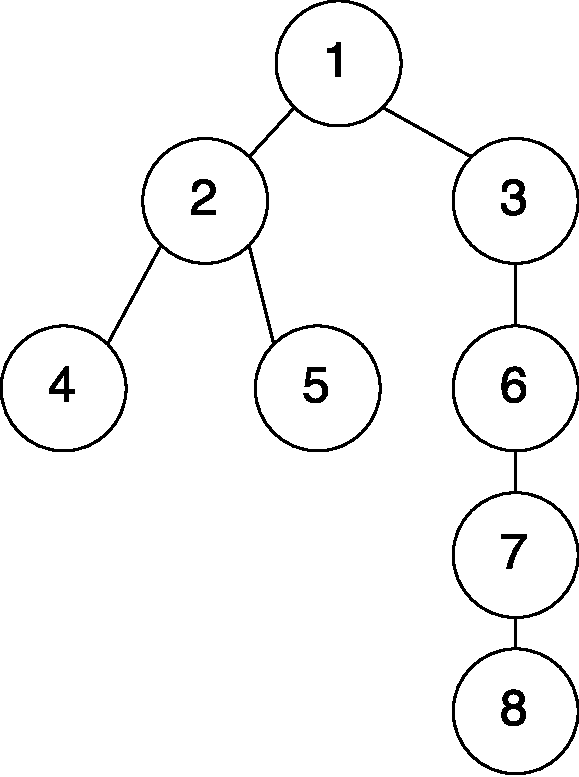
\includegraphics[width=0.28\textwidth]{ExampleTree}
  \caption{An example of an AST with nodes labeled for clarity.}
  \label{Fig:Tree}
\end{wrapfigure}

Figure \ref{Fig:Tree} shows an example AST, with its nodes numbered for reference. Using this tree we can compare different algorithms for selecting nodes, and see which best fulfils our requirements. Since we want to be able to add blanks to the model solution until the entire solution is blank, we should consider traversal algorithms. The algorithm will terminate when a node is selected to be made blank, and when it is next run it should (effectively) pick up from the same point. Since, clearly, the first choice of node to be replaced should be a leaf (any other choice would cause a larger percentage increase of the number of blank nodes, since such a node would have children that would simultaneously be made blank), some standard algorithms suggest themselves. The Depth First Traversal algorithm, when run on the example tree, would produce the output: 4,~5,~2,~8,~7,~6,~3,~1. Notice that node 2 is visited before node 8. This algorithm would concentrate all the blanks in the left hand side of the tree, reaching up to the left-most child of the root before considering the right hand side of the tree. This renders the Depth First Traversal algorithm unfit for our purposes. Another potential traversal algorithm to consider is the Reverse Level Order Traversal algorithm, which acts something like a Breadth First Traversal from the leaves upwards. When run on the example tree, this algorithm would produce the output: 8,~7,~4,~5,~6,~2,~3,~1. This algorithm suffers from a similar problem: node 7 is visited before node 4. This results in the blanks being concentrated on areas of the tree that have the deepest nodes, neglecting all other areas. This again means that the Reverse Level Order Traversal algorithm is not fit for our purposes. The ideal output for our algorithm would be as follows: 4,~5,~8,~2,~7,~6,~3,~1. This does a good job of distributing blanks across the tree without reaching the upper levels of the tree too soon. Since the tree is unbalanced, once we have visited node 2 we have no choice but to visit the long chain of nodes on the right hand side of the tree, but at least there are a decent number of blanks on both sides of the tree at that point. This output can be attained by a traversal algorithm that operates as described below, but before that it is worth making a somewhat subtle clarification. When describing these algorithms it has been useful to think of them as traversal algorithms, even though I would not be using them that way. At each execution of the algorithm, a single node is made blank. On the next execution, a different node will be made blank. After a finite number of executions, the entire solution will be blank. Since every node is selected exactly once, the combination of all the executions leading to an empty model solution can be considered a traversal of the tree. The following algorithm is difficult to describe as a simple traversal, since that is not its aim. As such, the following description includes directions to remove nodes from the tree, something that you definitely wouldn't find in a standard traversal. The simplest description of this algorithm comes with the appreciation that the purpose of the algorithm is in fact to replace nodes with blanks\footnote{Replacing a node with a blank is similar enough to deleting the node entirely that they can be interchangeable in this context. This is explained in the following paragraphs.}, not traverse the tree. With that in mind, here is a description of the ideal ``traversal'' algorithm:

\begin{enumerate}
\item{Traverse the tree as in the Depth First Traversal algorithm.}
\item{Whenever a leaf is reached, return that node, and remove it from the tree.}
\item{Repeat until the root has been removed.}
\end{enumerate}

It can be seen that this algorithm does indeed produce the desired output, 4,~5,~8,~2,~7,~6,~3,~1. During the first pass of the tree, the leaves labeled 4, 5, and 8 are returned and removed. Removing these leaves means that nodes 2 and 7 are now the leaves of the tree. On the next pass through, these leaves are returned and removed. The ``tree'' is now a simple chain of the nodes (returned in the order of bottom to top) 6, 3, 1.

The problem my algorithm must solve is more complex than a simple traversal. Not only should my algorithm terminate mid-traversal and be able to pick up from that point at the start of the next execution, but the process of actually inserting a blank into the tree is non-trivial, and not only that, but the results of executing the algorithm have to be reversed in order to replace a blank with the original code snippet. To see how I implemented the algorithm, found in the \texttt{addBlank} method of \texttt{AbstractPExercise}, let us begin by considering the simple problem and introduce more complexity as we go.

Since the first step is to traverse the tree as a Depth First Traversal, we must first implement this, using a \texttt{Stack<MiniJASTNode>} to store the nodes that still need to be dealt with. We start by pushing the root node (found in the \texttt{solution} field of the \texttt{AbstractPExercise} class) on to the nodes stack, as usual, and as usual we process this node before adding its children to the stack. Point 2 of the algorithm description says that when we find a leaf, we remove it from the tree. In the actual algorithm we wish to replace the node with a blank (the process for which I explain shortly), but since we are do not actually remove the node from the tree, we have a problem. Once we have made all the leaves of the tree blank, we have no more leaves to choose; this is in direct contrast to when we were simply removing leaves thereby creating more leaves. To fix this problem, we redefine the concept of leaves: a node is a leaf it has no children or all of its children are blank. In this way, by making leaves blank we are in fact creating more leaves. This definition of leaves is implemented in the \texttt{getIsLeaf} method declared in the \texttt{MiniJASTNode} interface and defined in the \texttt{ExpressionBase} and \texttt{StatementBase} abstract classes.

When we find a leaf, we wish to replace it with a blank. To do this, we have to replace the reference to the node in its parent with a reference to a new blank. At the moment, you cannot index nodes: you cannot access the $n$th child of a node, since they are simply stored in \texttt{private} fields. This means that it is very difficult to replace the reference to a child within a parent, without implementing a setter in every class that could translate the integer index to the appropriate field. This seems a lot more tiresome than simply allowing one to index nodes. To enable this, the \texttt{MiniJASTNode} interface declares the method \texttt{getSubNodes}, which returns \texttt{ArrayList<? extends MiniJASTNode>}. \texttt{StatementBase} and \texttt{ExpressionBase} both have a protected field, \texttt{subNodes}, which is returned by their overrides of this method. These fields are populated by the individual classes as their instances are set up. This means that rather than store their children directly as fields, each class in the implementation stores all its children in the \texttt{subNodes} field, and separately stores indexes into the array to provide access to the children during evaluation or execution. When we wish to replace a node with a blank, we store a blank at the appropriate index within its parent's \texttt{subNodes} field using the \texttt{getSubNodes} method. This means that we need to keep track of what the parent of the current node is, and also of the current node's index within its parents. These are stored in \texttt{Stack}s whose entries are updated as needed during the execution of the algorithm. 

Since we need to be able to undo the effects of an execution of the algorithm to be able to restore the original code, we need to store the nodes that were replaced as well as the list of indices giving the path through the tree to each node's original location. These are stored as \texttt{private} fields of the \texttt{AbstractPExercise} class, \texttt{Stack<MiniJASTNode>~replacedNodes} and \texttt{Stack<Stack<Integer>>~replacedNodeTreeIndices}. Whenever we replace a node, it is pushed onto the first stack, and the current stack of indices is pushed onto the second. The indices are also useful in enabling us to restart the algorithm where it left off. At the beginning of the algorithm, we check if the \texttt{replacedNodeTreeIndices} has any entries. If it does, we take the top one, reverse it (since the integer on top of the stack is the index of the last node in its parent and the integer on the bottom of the stack is the index of the root we need to follow first), and follow the indices through the tree. At each entry of the stack, we need to push the current node on to the parents stack, the index on to the index stack, and the children at and after, but not before, the index on to the nodes stack. The children after the index need to be pushed on too, as they have not yet been processed this pass of the tree.

In contrast to adding a blank, the algorithm that removes a blank from the model solution, \texttt{removeBlank} in \texttt{AbstractPExercise}, is much simpler. We simply take the top off the \texttt{replacedNodes} and \texttt{replacedNodeTreeIndices} stacks, follow the indices to the parent of the specific node, and use the last index to reinsert the node back in to its parents \texttt{subNodes} field.

This section described the implementation of the algorithms that introduce blanks to and remove them from a MiniJava program.

















\section{The \texttt{ExerciseSetter}}

In this section I describe how I made use of the language and its features to design the \texttt{ExerciseSetter}, one possible way in which students might interface with exercises designed to facilitate the learning of MiniJava.

The \texttt{ExerciseSetter} stores a list of possible exercises in order of increasing difficulty. The initial exercise to be delivered can be easily adjusted by changing the field \texttt{INITIAL\char`_EX}, and the current exercise index is also stored, along with a reference to that exercise. To measure the difficulty of the exercise and the performance of the students, the number of attempts at a solution made, the number of nodes in the solution, and the number of blanks added are also stored. A lot of the code in this class goes toward keeping these values consistent. The \texttt{ExerciseSetter} also stores a reference to an \texttt{OutputStream}, where all the output can be written to. This allows the \texttt{ExerciseSetter} to be plugged in to other peripherals, like the GUI described below. Finally, it also stores a reference to the parser.

A lot of the methods in this class are helper methods, simply passing messages between the exercise and the student. The important ones are \texttt{fillBlank}, \texttt{reportPerformance}, and \texttt{adjustQuestion}.

\texttt{fillBlank} has two method signatures, one that takes a \texttt{MiniJASTNode}, and one that takes a \texttt{String}. The one that takes a \texttt{MiniJASTNode} is trivial and thus unimportant, but the one that takes a \texttt{String} is more interesting. This method makes use of the parser in an interesting way, as there is of course some ambiguity in the language. The specific ambiguity comes from certain code snippets having the potential to be both \texttt{Expression}s and \texttt{Statement}s. An example of this is the code snippet \texttt{total = 1}. This can be parsed as an assignment, and would thus be classed an \texttt{Expression}, or a variable declaration, where the surrounding context might be \texttt{int total = 1;}, which would categorise this snippet as a \texttt{Statement}. To make the decision, the \texttt{ExerciseSetter} first checks if the blank being filled represents an \texttt{Expression} or a \texttt{Statement}, and sets the entry point for the parser appropriately.

\texttt{reportPerformance} is a possible implementation of a performance heuristic. Performance is based on the number of attempts the exercise took to solve, and the number of nodes in the solution compared with the model solution. The more attempts required and the more nodes in the solution, the worse the performance. A negative result here indicates that the next exercise should be easier, while a positive result indicates it should be harder.

\texttt{adjustQuestion} is a possible implementation of how the performance might influence the difficulty of the next problem. If the next exercise needs to be harder, then the \texttt{ExerciseSetter} adds blanks to the solution until either the exercise is hard enough, or the entire solution is blank. If the latter occurs, then the \texttt{ExerciseSetter} attempts to present a harder problem, and calculate how much of it should be blank. If instead the exercise needs to be easier, then the \texttt{ExerciseSetter} removes blanks from the solution until either the exercise is easy enough, or there are no blanks in the solution. If the latter occurs, then the \texttt{ExerciseSetter} attempts to present an easier problem and calculates how much of it should be blank.

In this section I have detailed one of the ways that students might interface with MiniJava through the \texttt{ExerciseSetter}. This is only an example of a possible use for the tools, but shows how powerful they can be.

\section{The GUI}

In this section I describe the implementation and function of the GUI peripheral.

\begin{figure}[h]
\centering
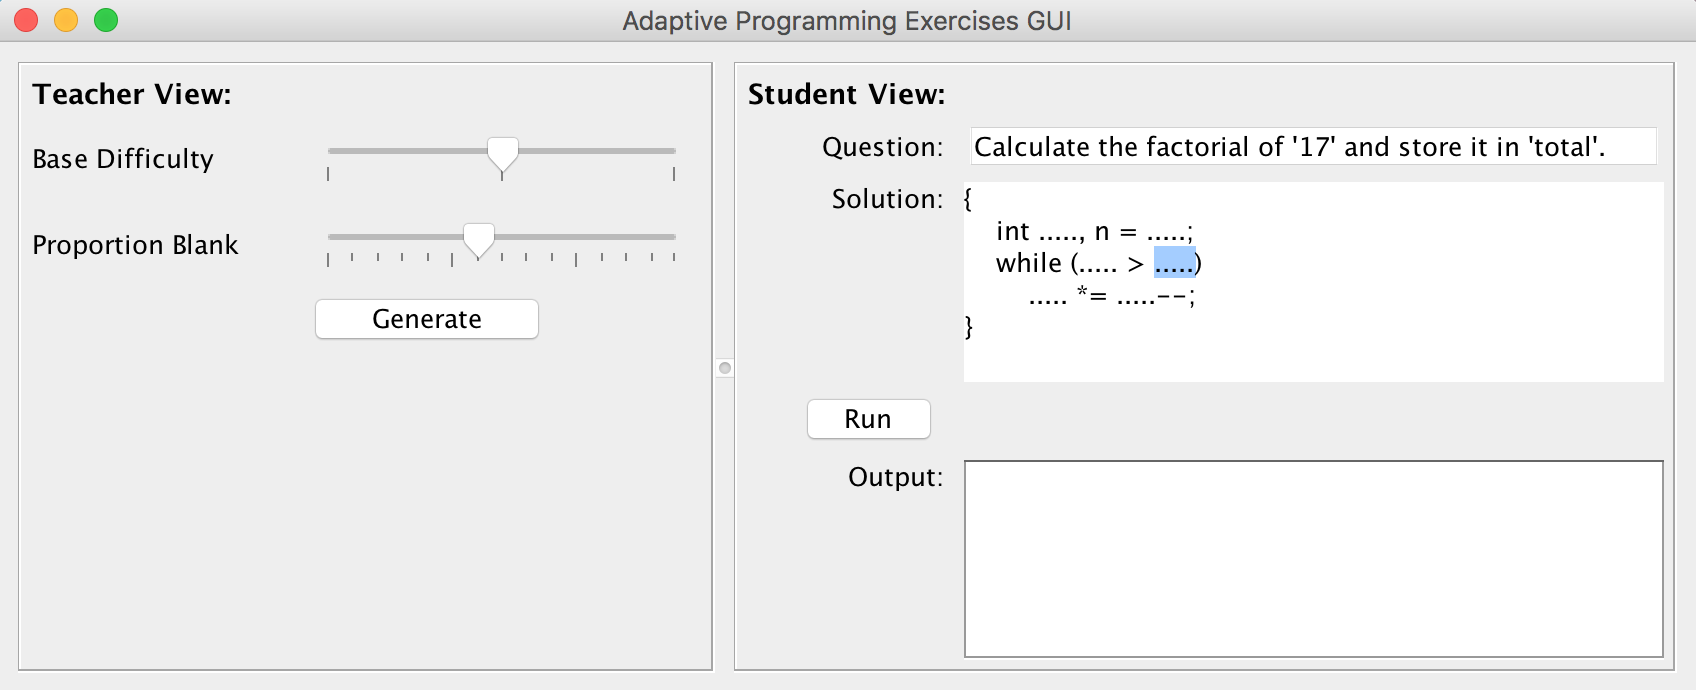
\includegraphics[width = \textwidth]{GUI}
\caption{An example screenshot taken of the GUI peripheral.}
\label{Fig:GUI}
\end{figure}

The GUI demonstrates some of the possible uses of this set of tools. It shows how a teacher might manually set the difficulty of a particular exercise and how a student could fill in the blanks and run their solution. An example screen from the GUI is shown in Fig 3. The top slider determines the problem that is presented: the further to the left the slider is, the easier the problem will be. The bottom slider affects the difficulty of that problem: the further it is to the left, the fewer blanks there will be and thus the easier the problem will be to solve. When the ``Generate'' button is pressed, the corresponding exercise will be displayed in the box on the right. 

When an exercise is generated, the blanks within the solution that need to be filled are shown as numbers in brackets surrounded by ellipses. To fill one of the blanks, the user must enter its number in the spinbox, and then enter the code with which to fill the blank in the text box, before pressing the button marked ``Fill Blank''. A blank with a given number can be emptied by entering its number into the spinbox and pressing the button marked ``Empty Blank''. The solution, i.e. the text in the large box on the right, can be executed at any time by pressing the ``Run'' button. The GUI will report whether the solution is correct or not.

The GUI was designed using the IntelliJ UI Designer plugin\footnote{https://www.jetbrains.com/help/idea/2017.1/swing-designing-gui.html}. This plugin allowed me to drag and drop components into place on the form before programming their functionality with the adjoining bound class. The class stores a reference to an \texttt{ExerciseSetter} object, which is where all the data comes from, and where the commands from the user are delivered to. It also makes use of the \texttt{ExerciseSetter}'s \texttt{setOutput} method by giving it a \texttt{ByteArrayOutputStream} that can then be read as text to be displayed. There is some error handling involved in that when something goes wrong, e.g. the user attempts to fill a blank with a number that isn't in the solution, or a solution run raises an error, the error is propagated up from the \texttt{ExerciseSetter} and displayed in the GUI.

This section described the function and then the implementation of the GUI peripheral.\\

In this chapter I have described what I have implemented and how I have done it. I started by giving the design of the language MiniJava, explaining some of these choices by introducing the parser and the concept of ``blanks'' within a MiniJava program. From there I explained how a programming exercise is conceptualised in the abstract sense, and gave an example of an implementation of a specific question. I finished by giving two possible uses for the set of tools, the \texttt{ExerciseSetter} and the Graphical User Interface (GUI).


\textcolor{red}{Estimated Word Count: 3765}

\chapter{Evaluation}

\chapter{Conclusion}

%%%%%%%%%%%%%%%%%%%%%%%%%%%%%%%%%%%%%%%%%%%%%%%%%%%%%%%%%%%%%%%%%%%%%
% the bibliography
\addcontentsline{toc}{chapter}{Bibliography}
\bibliography{refs}

%%%%%%%%%%%%%%%%%%%%%%%%%%%%%%%%%%%%%%%%%%%%%%%%%%%%%%%%%%%%%%%%%%%%%
% the appendices
\appendix

\chapter{The Parser}
\label{App:Parser}

\begin{Verbatim}[tabsize=4]
grammar MiniJava;

// STATEMENTS / BLOCKS

// entry point
entry
	: block [true]			# blockEntry
	| blockStatement+		 # blockStatementsEntry
	| statementTop			# statementEntry
	| expression			  # expressionEntry
	;									

block [boolean isOuter]
	: LBRACE blockStatement* RBRACE						
	;

blockStatement
	: primitiveType variableDeclarators SEMI	# localVariableDeclaration
	| statement								 # makeStmnt
	| variableDeclarator					    # makeVarDec
	;
    
statementTop
	: statement					   # stmnt
	| statementNSI					# stmntNSI
	;

\end{Verbatim}
\begin{Verbatim}[samepage=true, tabsize=4]
statement
	: block [false]									 # makeBlock
	| IF parExpression statement 					   # makeIf
	| IF parExpression statementNSI ELSE statement	  # makeITE
	| FOR LPAREN forInit? SEMI expression? 
		SEMI expressionList? RPAREN  statement		  # makeFor
	| WHILE parExpression statement					 # makeWhile
	| statementNTS									  # makeStatementNTS
	;
\end{Verbatim}

\begin{Verbatim}[tabsize=4]  
statementNSI
	: block [false]									  # makeBlockNSI
	| IF parExpression statementNSI ELSE statementNSI	# makeITENSI
	| FOR LPAREN forInit? SEMI expression? 
		SEMI expressionList? RPAREN statementNSI 		# makeForNSI
	| WHILE parExpression statementNSI				   # makeWhileNSI
	| statementNTS									   # makeStatementNTSNSI												
	;
    
statementNTS
	: DO statement WHILE parExpression SEMI	  # makeDo
	| RETURN SEMI								# return
	| BREAK SEMI								 # break
	| CONTINUE SEMI							  # continue
	| SEMI									   # empty
	| expressionStatement SEMI				   # makeStmntExpr
	;


forInit
	: primitiveType variableDeclarators			 # forInitLVD
	| expressionList								# forInitExprs
	;

// EXPRESSIONS

parExpression
	: LPAREN expression RPAREN
	;

expressionList
	: expression (COMMA expression)*
	;

expressionStatement
	: expression
	;

expression // Most binding comes first!
	: Identifier											   # makeID
	| expression LBRACK expression RBRACK					  # arrayAccess
	| parExpression										    # makeBracketed
	| literal												  # makeLiteral
	| expression (op=INC | op=DEC)							 # postInc
	| (op=ADD|op=SUB|op=INC|op=DEC) expression				 # preIncEtc
	| BANG expression										  # makeNot
	| expression (op=MUL|op=DIV) expression				    # multExpr
	| expression (op=ADD|op=SUB) expression			  	  # addExpr
	| expression (op=LE | op=GE | op=GT | op=LT) expression	# relationalExpr
	| expression (op=EQUAL | op=NOTEQUAL) expression		   # eqExpr
	| expression AND expression								# andExpr
	| expression OR expression								 # orExpr
	| <assoc=right> expression QUESTION 
		expression COLON expression						    # condExpr
	| <assoc=right> expression												
		(   op=ASSIGN
        		|   op=ADD_ASSIGN
        		|   op=SUB_ASSIGN
        		|   op=MUL_ASSIGN
        		|   op=DIV_ASSIGN
        		)
        		expression									 # assignExpr
	;
    
// VARIABLES AND LITERALS
    
variableDeclarators
	: variableDeclarator (COMMA variableDeclarator)*
	;

variableDeclarator
	: Identifier LBRACK RBRACK (ASSIGN variableInitializer)?   # arrayVarDec 
	| Identifier (ASSIGN variableInitializer)?				 # singleVarDec
	;
\end{Verbatim}
\begin{Verbatim}[samepage=true,tabsize=4]
variableInitializer 
	: arrayInitializerValues								   # arrayInitVals
	| arrayInitializerSize									 # arrayInitSize
	| expression											   # initExpr
	;
\end{Verbatim}
\begin{Verbatim}[tabsize=4]
arrayInitializerValues
	: LBRACE variableInitializer (COMMA variableInitializer)* (COMMA)? RBRACE	
	;
    
arrayInitializerSize
	: NEW primitiveType LBRACK expression RBRACK
	;

primitiveType
	: BOOLEAN
	| CHAR
	| INT
	| DOUBLE
	;

literal
	: IntegerLiteral 
	| FloatingPointLiteral 
	| CharacterLiteral
	| BooleanLiteral
	;

// LEXER
// �3.9 Keywords

BOOLEAN	    : 'boolean';
BREAK		  : 'break';
CHAR		   : 'char';
CONTINUE	   : 'continue';
DO			 : 'do';
DOUBLE		 : 'double';
ELSE		   : 'else';
FOR			: 'for';
IF			 : 'if';
INT			: 'int';
NEW			: 'new';
RETURN		 : 'return';
WHILE		  : 'while';

// �3.10.1 Integer Literals
// �3.10.2 Floating-Point Literals
// �3.10.3 Boolean Literals
// �3.10.4 Character Literals
// �3.11 Separators
// Sections removed for clarity

LPAREN          : '(';
RPAREN          : ')';
LBRACE          : '{';
RBRACE          : '}';
LBRACK          : '[';
RBRACK          : ']';
SEMI            : ';';
COMMA           : ',';
DOT             : '.';

// �3.12 Operators

ASSIGN          : '=';
GT              : '>';
LT              : '<';
BANG            : '!';
QUESTION        : '?';
COLON           : ':';
EQUAL           : '==';
LE              : '<=';
GE              : '>=';
NOTEQUAL        : '!=';
AND             : '&&';
OR              : '||';
INC             : '++';
DEC             : '--';
ADD             : '+';
SUB             : '-';
MUL             : '*';
DIV             : '/';

ADD_ASSIGN      : '+=';
SUB_ASSIGN      : '-=';
MUL_ASSIGN      : '*=';
DIV_ASSIGN      : '/=';

// �3.8 Identifiers (must appear after all keywords in the grammar)
//
// Whitespace and comments
//
// Sections removed for clarity
\end{Verbatim}

\chapter{Project Proposal}

% Note: this file can be compiled on its own, but is also included by
% diss.tex (using the docmute.sty package to ignore the preamble)
\documentclass[12pt,a4paper,twoside]{article}
\usepackage[pdfborder={0 0 0}]{hyperref}
\usepackage[margin=25mm]{geometry}
\usepackage{graphicx}
\usepackage{parskip}
\begin{document}

\begin{center}
\Large
Computer Science Tripos -- Part II -- Project Proposal\\[4mm]
\LARGE
A System for Giving Programming Exercises \\Adaptive Difficulty\\[4mm]

\large
R.~J.~McFarland, Homerton College

Originator: M.~B.~Gale

20 October 2016
\end{center}

\vspace{5mm}

\textbf{Project Supervisor:} M.~B.~Gale

\textbf{Director of Studies:} Dr J.~Fawcett

\textbf{Project Overseers:} Dr D.~J.~Greaves  \& Prof J.~G.~Daugman

% Main document

\section*{Introduction}

Different people learn at different speeds, and learn some things more quickly than others. When a group of students are given a set of programming exercises, this typically isn't taken account of. The aim of this project is to design a system that varies the difficulty of a programming exercise depending on how the individual has performed completing previous exercises. 

The difficulty of an exercise can be measured using two metrics: how complex the problem being solved is and how much code the student is expected to write. The system will vary both of these to adapt the difficulty of proposed exercises automatically (i.e. the system will not look for preprogrammed mistakes, but rather interpret the mistakes made and react accordingly). When an exercise is completed to a sufficient standard, a similar exercise will be given, but expecting more code to be written. When the system has determined that the problem has been mastered, a more difficult problem will be presented, requiring less code to be written again.

\section*{Resources required}

I shall use my own Macintosh laptop for the majority of this project. Backup will be to GitHub and to a 5TB hard drive I keep in my room. I shall make use of the Java standard library, as well as the JavaFX library for the graphical user interface element. I require no special resources.

\section*{Starting point}

I am able to program in Java, and have used JavaFX before for the Part IB group project. During my A-Levels I wrote a program to test the maths abilities of Year 4 students, which involved the programmatic generation of various kinds of maths questions.

\section*{Work to be done}

The work for this project can be split up into the following sub-projects:
\begin{enumerate}
\item{A representation of a programming exercise must be coded up to allow the final product to manipulate them.}
\item{A heuristic that measures the difficulty of a given exercise must be chosen and implemented.}
\item{A heuristic that assesses how well a ``student'' has completed an exercise must be chosen and implemented.}
\item{I must devise a system, using the previous three items, that determines which exercise should be given to the student next, as well as how much of the required code is already filled in, based on the student's performance completing previous exercises.}
\item{A Graphical User Interface should be designed to enable a user to manually adjust the content of a given programming exercise.}
\item{In order to test the program, a student will be simulated by creating a system that tells the program what errors were made where and how long the exercise took to be solved, so that the program's response to various stimuli can be measured.}
\end{enumerate}

\section*{Success Criteria}

The project will be considered completed when:
\begin{enumerate}
\item{I have a system that presents the same initial problem to all students.}
\item{The system can determine that code written by the student solves the given problem.}
\item{On registering completion of the exercise, the system will then present a new problem to the student.}
\item{If the student solved this problem with sufficient ease as measured by my performance heuristic, then this new problem will be more difficult, as measured by my difficulty heuristic.}
\item{If the student failed to solve the problem, or took too much time or made too many errors, then the next problem will be easier.}
\item{The system will adjust the difficulty of a given problem in line with the difficulty heuristic by changing the amount of code required to solve the problem, and also the underlying problem being solved.}
\end{enumerate}

\section*{Possible extensions}

\begin{itemize}
\item{This system could be improved such that it identifies which concepts a student is struggling with and adjusts the content of future exercises to encourage learning of these concepts.}
\item{The program could produce a graph of progress against time to motivate learners.}
\item{A simple game that utilises this system could be made, to showcase how the system might be used to teach programming.}
\end{itemize}

\section*{Timetable}

\textbf{24th Oct - 6th Nov:} 
\begin{itemize}
\item{Research adaptive difficulty and see how it has been done before.}
\item{Research how errors in code have been quantified in the past.}
\item{Research where and how simulated users have been designed to test systems.}
\end{itemize}

\textbf{7th Nov - 20th Nov:}
\begin{itemize}
\item{Describe how code that solves an exercise could be split up into discrete sections, and a way to store how well each of those sections was completed.}
\end{itemize}
\underline{Milestones:}
\begin{itemize}
\item{Have a representation of a programming puzzle in Java code.}
\end{itemize}

\textbf{21st Nov - 4th Dec:}
\begin{itemize}
\item{Prototype and compare heuristics to measure the ``difficulty'' of a given programming exercise, based on the difficulty of the goal to be achieved, and how much of the code is presented initially.}
\end{itemize}
\underline{Milestones:}
\begin{itemize}
\item{Select and implement a difficulty heuristic.}
\end{itemize}

\textbf{5th Dec - 18th Dec:}
\begin{itemize}
\item{Prototype and compare heuristics to measure performance, based perhaps on how much time was taken, the number of errors made and the time the solution takes to run.}
\end{itemize}
\underline{Milestones:}
\begin{itemize}
\item{Select and implement a performance heuristic.}
\end{itemize}

\textbf{19th Dec - 1st Jan:}
\begin{itemize}
\item{Slack time over Christmas to catch up if I need to.}
\end{itemize}

\textbf{2nd Jan - 15th Jan:}
\begin{itemize}
\item{Implement a system to adapt the difficulty of the programming exercises by presenting a new, more difficult problem each time an exercise is completed satisfactorily, and presenting an easier one if the student is struggling too much.}
\end{itemize}
\underline{Milestones:}
\begin{itemize}
\item{Have a system that will present a problem to a student, determine that the student has solved the problem with the code they have written, determine if the student found it too easy or too hard, and present the student with a new problem that is either easier or harder respectively.}
\end{itemize}

\textbf{16th Jan - 29th Jan:}
\begin{itemize}
\item{Write Progress Report.}
\item{Improve the system by implementing the concept of changing the amount of code that needs to be written to solve a given problem as another way of affecting its difficulty.}
\end{itemize}
\underline{Milestones:}
\begin{itemize}
\item{Have the system extended such that it may require the student to write more or less code to make more fine grained adjustments to the difficulty of a programming problem.}
\end{itemize}

\textbf{30th Jan - 19th Feb:}
\begin{itemize}
\item{\textbf{3rd Feb:} Submit the Progress Report}
\item{Design a user interface to change the content of the programming exercise to be solved.}
\end{itemize}
\underline{Milestones:}
\begin{itemize}
\item{Have a user interface with controls to determine the exact difficulty of the problem about to be presented.}
\end{itemize}

\textbf{20th Feb - 5th Mar:}
\begin{itemize}
\item{Write unit tests for all units.}
\end{itemize}
\underline{Milestones:}
\begin{itemize}
\item{Have unit tests written for every unit of the code.}
\end{itemize}

\textbf{6th Mar - 19th Mar:}
\begin{itemize}
\item{Test the implementation by simulating a student ``using'' the system by ``solving'' problems with varying success.}
\end{itemize}
\underline{Milestones:}
\begin{itemize}
\item{Have a simulated student that will tell the system what mistakes were made in the code and where, as well as how long it took to solve the problem (along with any other parameters deemed important to measuring the performance of the student), such that the response of my system can be measured against the performance of a student using it.}
\end{itemize}

\textbf{20th Mar - 2nd Apr:}
\begin{itemize}
\item{Slack time for catching up and doing extensions.}
\end{itemize}

\textbf{3rd Apr - 16th Apr:}
\begin{itemize}
\item{Write Introduction and Conclusion (about 2,500 words).}
\item{Write up Proforma (excluding word count), Declaration of Originality, Project Proposal and Cover Sheet.}
\end{itemize}
\underline{Milestones:}
\begin{itemize}
\item{Have the above sections of the dissertation written in draft form.}
\end{itemize}


\textbf{17th Apr - 30th Apr}
\begin{itemize}
\item{Write Preparation and Implementation (about 5000 words).}
\end{itemize}
\underline{Milestones:}
\begin{itemize}
\item{Have the above sections of the dissertation written in draft form.}
\end{itemize}

\textbf{1st May - 14th May}
\begin{itemize}
\item{Write Evaluation (about 2500 words).}
\item{Write Contents Page, finish Bibliography, Appendices and Index as required.}
\item{Fill in word count of Proforma.}
\item{Submit draft to DoS and Supervisor.}
\end{itemize}
\underline{Milestones:}
\begin{itemize}
\item{Have the above sections of the dissertation written in draft form.}
\end{itemize}

\textbf{15th May - 19th May}
\begin{itemize}
\item{Incorporate feedback into dissertation.}
\item{\textbf{19th May:} Submit dissertation.}
\end{itemize}


\end{document}

\end{document}
